% As part of the assignment on ML Testing, you had to design a testing strategy and implement
% some automated tests. In this section, we expect you to fully document your choices and to reflect on limitations of the existing testing strategy. Moreover, we would like to hear your thoughts on how to improve tests, which new tests should be implemented and why.

\section{ML Testing Design}
In order to verify our entire systems functions correctly, reliably and effectively, we have set up an extensive Continuous Integration (CI) pipeline. This pipeline consists of five steps: installing dependencies, installing and configuring \hyperref[sec:ml-pipeline:dvc]{DVC}, running tests, running benchmarks and running \hyperref[sec:ml-pipeline:lint]{linting}. This workflow is visualised in Figure \ref{fig:ci-pipeline}. The following sections will elaborate on the testing and benchmark steps.

\begin{figure*}[h]
    \centering
    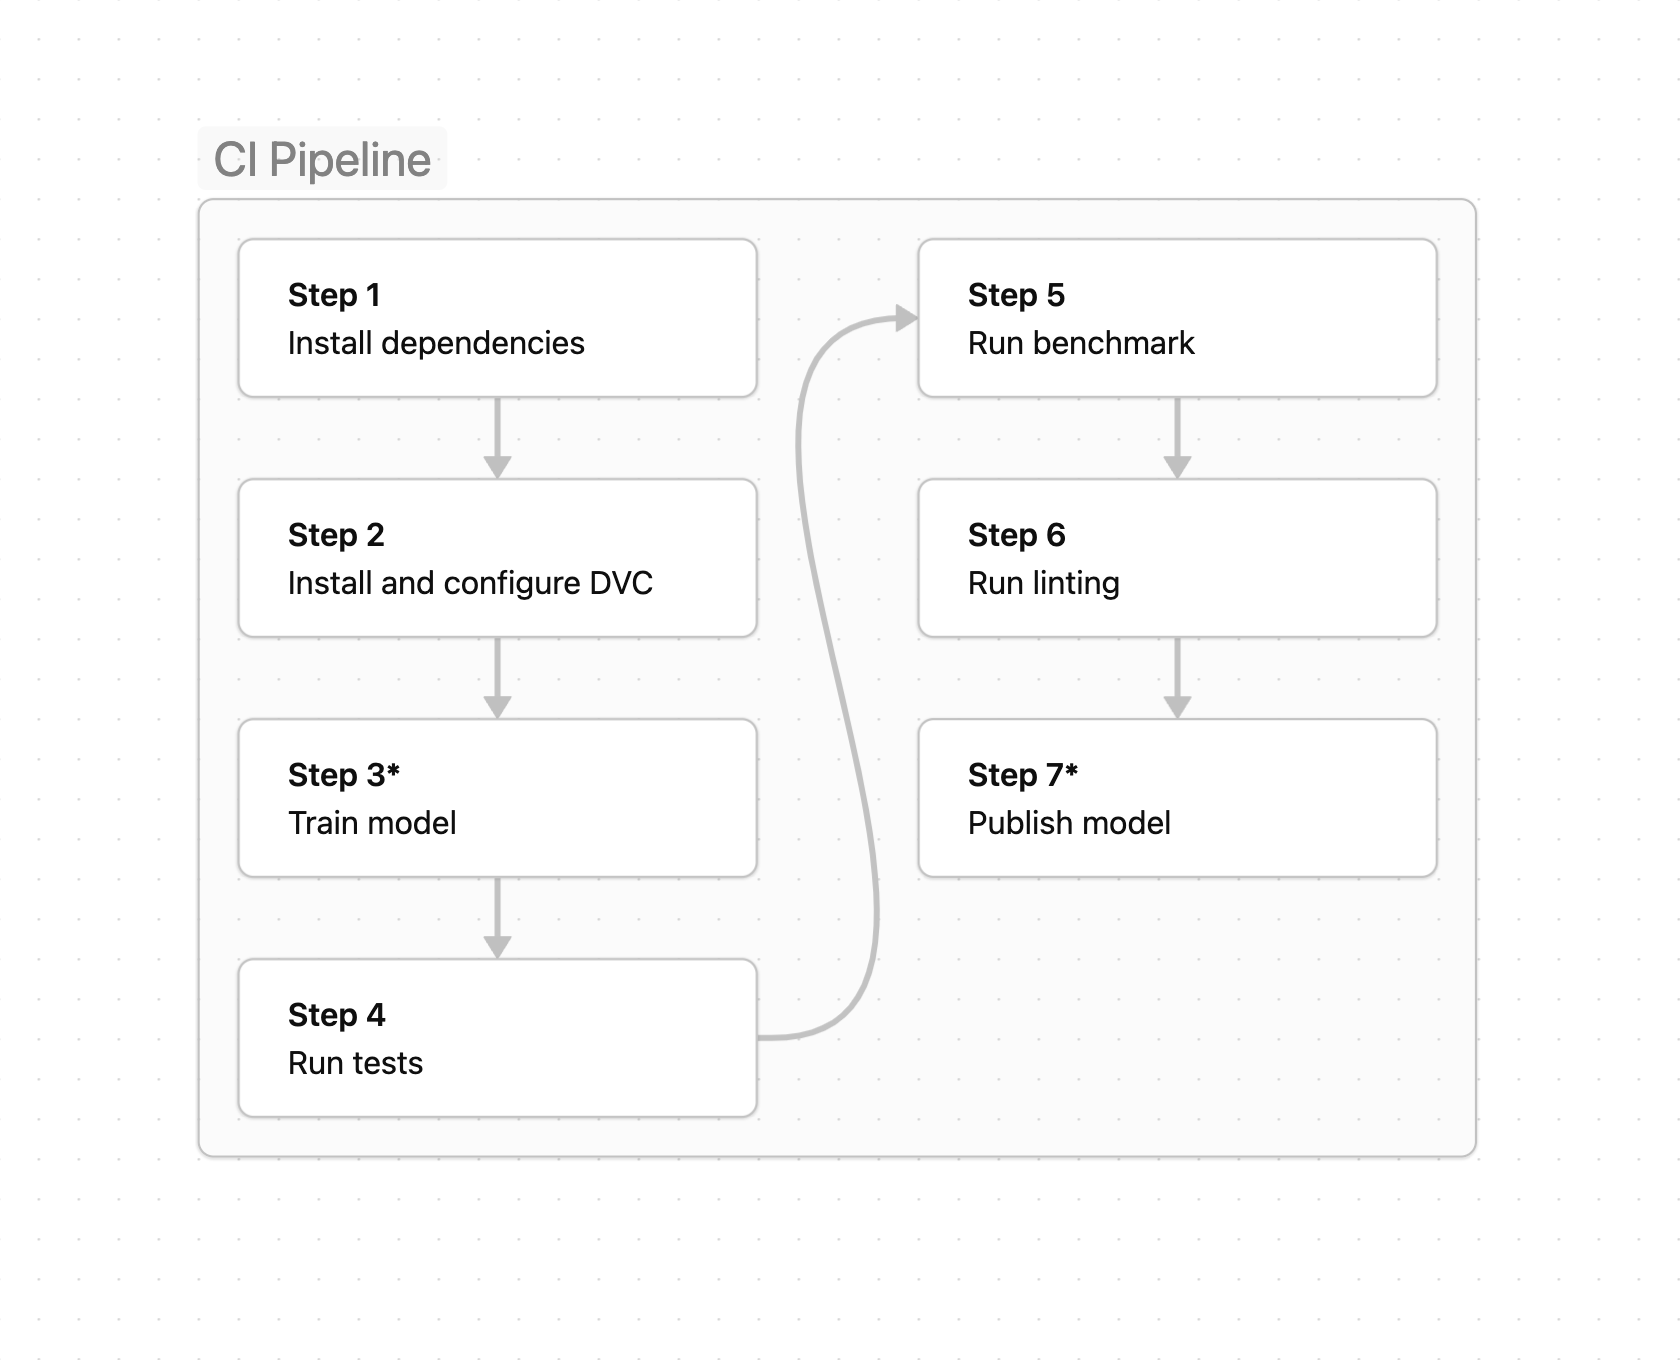
\includegraphics[width=\textwidth]{images/ci_pipeline.png}
    \caption{Continuous Pipeline steps}
    \label{fig:ci-pipeline}
\end{figure*}

\subsection{Test Strategy}
Our testing strategy was guided by the paper \textit{What’s your ML Test Score? A rubric for ML production systems}\cite{mltestscore}. Four main aspects of ML testing are outlined, as well as a system of computing an ML test score. We have implemented the following tests based on these aspects:

\subsubsection{Tests for Features and Data:} Since the behaviour of ML systems learned from data, it is important to verify that the data delivered and handled as expected. We have implemented tests to verify that all steps in the DVC pipeline create correct output files. Additionally, the input features are checked for duplicate data.

\subsubsection{Tests for Model Development}
TODO

\subsubsection{Tests for ML Infrastructure:} To test the ML infrastructure, we are testing the reproducibility of training the model. The model is trained two times on the same data, but with different seeds. We can detect non-determinism when the accuracy of these models differs more than a threshold.

\subsubsection{Monitoring Tests for ML:} To monitor how our ML pipeline performs, we have implemented a benchmark using \textit{PyTest Benchmark}\footnote{https://pypi.org/project/pytest-benchmark/}. Paired with the GitHub Action \textit{github-action-benchmark}\footnote{https://github.com/benchmark-action/github-action-benchmark/tree/master}, the performance of training the model is automatically measured and compared to previous runs. If the change is too drastic, the pipeline will raise an error.

Since a lot of the tests involve training the model, the full CI pipeline takes quite a long time to run. This is not preferable during development, where quick feedback is key to fast iterating and bug-fixing. To mitigate this problem, we have decided to split up the pipeline into two versions based on how they are triggered:

\begin{enumerate}
    \item \textit{Pull requests:} When a pull request is opened, the pipeline will be ran on a random 10\% sample of the dataset. This will allow for quick feedback with reasonably accurate test results.
    \item \textit{Pushes to main:} When a push is made to the main branch, the pipeline will be ran on the full dataset. This can be used as a final verification after a pull request has been merged.
\end{enumerate}

\subsection{Improvements}
TODO